\section{Casi d'uso}\label{sec:casi-d'uso}
Di seguito sono elencati i casi d'uso individuati dallo stagista durante la fase dell'analisi dei requisiti.
\subsection*{UC-1 Selezione file}\label{subsec:uc-1-selezione-file}
\begin{itemize}
    \item \textbf{attori:} utente generico;
    \item \textbf{descrizione:} serve per permettere all'utente di selezionare il file APK da analizzare;
    \item \textbf{pre-condizioni:} l'utente ha avviato il tool;
    \item \textbf{post-condizioni:} l'utente ha selezionato un file di estensione APK valido;
    \item \textbf{flusso degli eventi principali:}
    \begin{itemize}
        \item l'utente seleziona il file;
        \item l'utente conferma la selezione del file.
    \end{itemize}
\end{itemize}
\subsection*{UC-2 Avvio decompilazione}\label{subsec:uc-2-avvio-decompilazione}
\begin{itemize}
    \item \textbf{attori:} utente generico;
    \item \textbf{descrizione:} l'utente deve avviare la decompilazione del file APK;
    \item \textbf{pre-condizioni:} l'utente ha selezionato con successo un file APK;
    \item \textbf{post-condizioni:} la decompilazione è avvenuta con successo;
    \item \textbf{flusso degli eventi principali:}
    \begin{itemize}
        \item l'utente avvia la decompilazione;
        \item l'utente visualizza il messaggio della decompilazione avvenuta con successo;
    \end{itemize}
    \item \textbf{Estensione:}
    \begin{itemize}
        \item UC-3 Visualizzazione errore di decompilazione;
    \end{itemize}
\end{itemize}

\subsection*{UC-3 Visualizzazione errore di decompilazione}\label{subsec:uc-3-visualizzazione-errore-di-decompilazione}
\begin{itemize}
    \item \textbf{attori:} utente generico;
    \item \textbf{descrizione:} la decompilazione del file APK potrebbe generare degli errori;
    \item \textbf{pre-condizioni:} l'utente ha avviato la decompilazione dell'APK;
    \item \textbf{post-condizioni:} l'utente ha visualizzato il messaggio d'errore;
    \item \textbf{flusso degli eventi principali:}
    \begin{itemize}
        \item l'utente visualizza il messaggio di errore;
    \end{itemize}
\end{itemize}
\subsection*{UC-4 Installazione APK ricompilato}\label{subsec:uc-4-installazione-apk-decompilato}
\begin{itemize}
    \item \textbf{attori:} utente generico;
    \item \textbf{descrizione:} permette all'utente d'installare l'apk, decompilato, modificato e ricompilato, su un AVD;
    \item \textbf{pre-condizioni:} la decompilazione dell'APK è stata eseguita con successo;
    \item \textbf{post-condizioni:} l'APK è stato installato sull'AVD con successo;
    \item \textbf{flusso degli eventi principali:}
    \begin{itemize}
        \item l'utente seleziona un'AVD presente sul proprio computer;
        \item l'utente avvia l'installazione dell'APK ricompilato;
        \item l'utente visualizza un messaggio che segnala l'installazione avvenuta con successo.
    \end{itemize}
\end{itemize}
\subsubsection*{UC-4.1 Selezione AVD}\label{subsubsec:uc-4.1-selezione-avd}
\begin{itemize}
    \item \textbf{attori:} utente generico;
    \item \textbf{descrizione:} serve per permettere all'utente di selezionare un'AVD presente nel proprio computer;
    \item \textbf{pre-condizioni:} l'utente ha avviato lo strumento;
    \item \textbf{post-condizioni:} l'utente ha selezionato l'AVD da avviare;
    \item \textbf{flusso degli eventi principali:}
    \begin{itemize}
        \item l'utente visualizza un elenco delle AVD presenti nel proprio computer;
        \item l'utente seleziona un'AVD;
        \item l'utente conferma la selezione;
        \item l'AVD selezionato si è avviato con successo.
    \end{itemize}
    \item \textbf{Estensione}
    \begin{itemize}
        \item UC-5 Visualizzazione messaggio nessun AVD rilevato;
    \end{itemize}
\end{itemize}
\begin{figure}
    \centering
    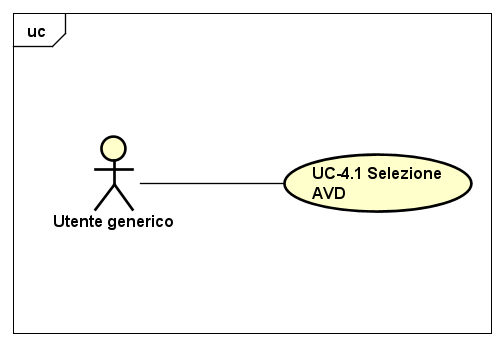
\includegraphics[width=10cm, height=8cm]{./usecase/uc_4_1.png}
    \caption{Sottocaso d'uso UC-4.1 Selezione AVD.}
\end{figure}

\subsection*{UC-5 Visualizzazione messaggio nessun AVD rilevato} \label{subsec:uc-5-visualizzazione-messaggio-nessun-avd-rilevato}
\begin{itemize}
    \item \textbf{attori:} utente generico;
    \item \textbf{descrizione:} quando non sono presenti nessun AVD o il tool non è riuscito a rilevarne, viene mostrato un messaggio all'utente;
    \item \textbf{pre-condizioni:} l'utente ha aperto il tool;
    \item \textbf{post-condizioni:} l'utente ha visualizzato il messaggio;
    \item \textbf{flusso degli eventi principali:}
    \begin{itemize}
        \item l'utente visualizza il messaggio;
    \end{itemize}
\end{itemize}
\subsection*{UC-6 Errore durante avvio dell'AVD}\label{subsec:uc-6-errore-durante-avvio-dell'avd}
\begin{itemize}
    \item \textbf{attori:} utente generico;
    \item \textbf{descrizione:} serve a mostrare all'utente gli eventuali errori durante l'avvio dell'AVD;
    \item \textbf{pre-condizioni:} l'utente ha selezionato un'AVD e ha confermato l'avvio;
    \item \textbf{post-condizioni:} l'utente ha visualizzato il messaggio d'errore;
    \item \textbf{flusso degli eventi principali:}
    \begin{itemize}
        \item l'utente visualizza il messaggio d'errore;
    \end{itemize}
\end{itemize}
\subsection*{UC-7 Dump dello storage interno}\label{subsec:uc-6-dump-dello-storage-interno}
\begin{itemize}
    \item \textbf{attori:} utente generico;
    \item \textbf{descrizione:} nel caso l'utente volesse una copia dei dati interni dell'applicativo, ha bisogno di fare il dump;
    \item \textbf{pre-condizioni:} l'installazione dell'APK modificato è andata a buon fine;
    \item \textbf{post-condizioni:} l'area di storage dell'app è stata copiata con successo;
    \item \textbf{flusso degli eventi principali:}
    \begin{itemize}
        \item l'utente seleziona la voce "copia i dati interni";
        \item l'utente seleziona il path dove collocare i dati.
    \end{itemize}
\end{itemize}
\subsection*{UC-8 Decodifica del codice}\label{subsec:uc-8-decodifica-del-codice}
\begin{itemize}
    \item \textbf{attori:} utente generico;
    \item \textbf{descrizione:} durante la decompilazione dell'APK vengono creati dei file .dex che contengono il codice sorgente dell'APK, e questo caso d'uso serve per permettere all'utente di ottenere il codice sorgente;
    \item \textbf{pre-condizioni:} la decompilazione è avvenuta con successo;
    \item \textbf{post-condizioni:} l'utente ha ottenuto una copia del codice sorgente in java;
    \item \textbf{flusso degli eventi principali:}
    \begin{itemize}
        \item l'utente ha selezionato la funzionalità di decodifica dei dex;
        \item l'utente seleziona il percorso dove posizionare il codice sorgente ottenuto;
        \item l'utente ha salvato il codice sorgente ottenuto.
    \end{itemize}
\end{itemize}
\subsubsection*{UC-8.1 Avvio decodifica}
\begin{itemize}
    \item \textbf{attori:} utente generico;
    \item \textbf{descrizione:} serve all'utente per avviare la decodifica dei file .dex;
    \item \textbf{pre-condizioni:} la decompilazione dell'APK è avvenuta correttamente;
    \item \textbf{post-condizioni:} la decodifica è avvenuta con successo;
    \item \textbf{flusso degli eventi principali:}
    \begin{itemize}
        \item l'utente seleziona la funzionalità di decodifica dei file .dex;
    \end{itemize}
\end{itemize}
\subsubsection*{UC-8.2 Salvataggio del codice decodificato}
\begin{itemize}
    \item \textbf{attori:} utente generico;
    \item \textbf{descrizione:} serve all'utente per salvare i codici sorgenti decodificati;
    \item \textbf{pre-condizioni:} la decompilazione è avvenuta con successo;
    \item \textbf{post-condizioni:} i file con i codici sorgenti sono stati salvati correttamente;
    \item \textbf{flusso degli eventi principali:}
    \begin{itemize}
        \item l'utente seleziona la voce "salva file decodificati";
        \item l'utente seleziona la posizione dove vuole salvare i file;
        \item i file vengono salvati correttamente.
    \end{itemize}
\end{itemize}

\begin{figure}[H]
    \centering
    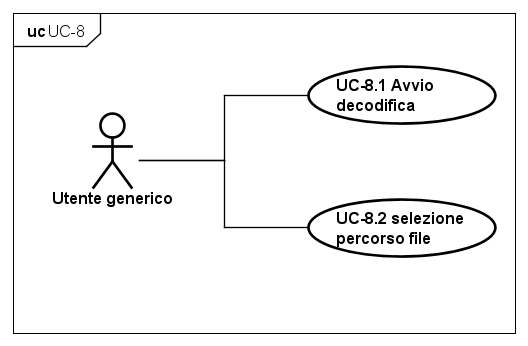
\includegraphics[width=10cm, height=8cm]{./immagini/usecase/uc_8.png}
    \caption{Caso d'uso UC-8 Decodifica codici .dex.}
\end{figure}



\subsection*{UC-9 Visualizzazione errore decodifica}\label{subsec:uc-9-visualizzazione-errore-decodifica}
\begin{itemize}
    \item \textbf{attori:} utente generico;
    \item \textbf{descrizione:} durante la decodifica dei .dex possono sorgere molteplici errori;
    \item \textbf{pre-condizioni:} l'utente ha selezionato la funzionalità di decodifica del codice .dex;
    \item \textbf{post-condizioni:} l'utente ha visualizzato il messaggio di errore durante la decodifica;
    \item \textbf{flusso degli eventi principali:}
    \begin{itemize}
        \item l'utente ha visualizzato il messaggio d'errore;
    \end{itemize}
\end{itemize}

\begin{figure}[H]
    \centering
    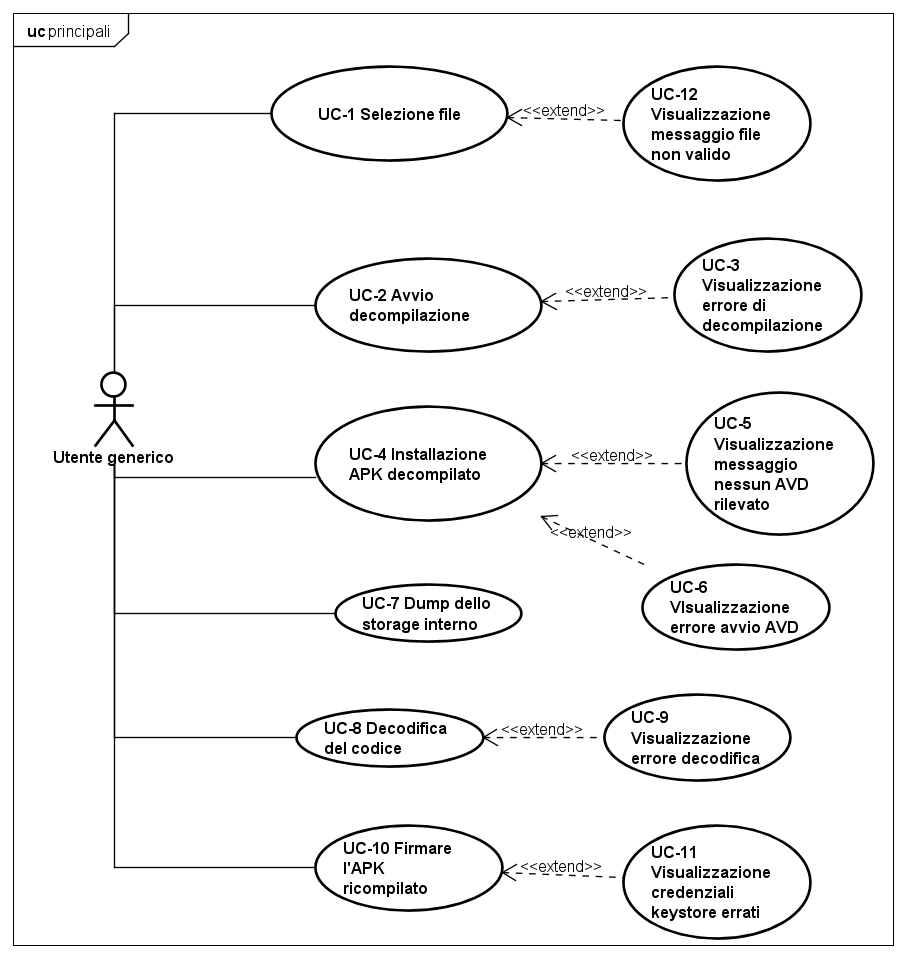
\includegraphics[width=10cm, height=8cm]{./immagini/usecase/uc_principali.png}
    \caption{Casi d'uso da 1 a 12.}
\end{figure}

\subsection*{UC-10 Firmare l'APK ricompilato}\label{subsec:uc-10-firmare-l'apk-ricompilato}
\begin{itemize}
    \item \textbf{attori:} utente generico;
    \item \textbf{descrizione:} dopo la ricompilazione si può firmare l'APK;
    \item \textbf{pre-condizioni:} la ricompilazione dell'APK è avvenuta correttamente;
    \item \textbf{post-condizioni:} l'APK è stata firmato correttamente;
    \item \textbf{flusso degli eventi principali:}
    \begin{itemize}
        \item UC-10.1 selezione keystore;
        \item UC-10.3 inserimento alias;
        \item UC-10.4 inserimento password.
    \end{itemize}
    \item \textbf{Estensione}
    \begin{itemize}
        \item UC-11 Visualizzazione credenziali keystore errate;
    \end{itemize}
\end{itemize}
\subsubsection*{UC-10.1 Selezione keystore}\label{subsubsec:uc-10.1-selezione-keystore}
\begin{itemize}
    \item \textbf{attori:} utente generico;
    \item \textbf{descrizione:} l'utente deve selezionare il keystore da utilizzare per firmare l'APK
    \item \textbf{pre-condizioni:} la ricompilazione dell'APK è avvenuta correttamente;
    \item \textbf{post-condizioni:} è stato selezionato un file di tipo keystore corretto (estensione: \textbf{.jks});
    \item \textbf{flusso degli eventi principali:}
    \begin{itemize}
        \item l'utente seleziona la funzionalità per selezionare il keystore;
        \item l'utente seleziona il keystore;
    \end{itemize}
    \item \textbf{flussi secondari}
    \begin{itemize}
        \item UC-10.2 visualizzazione messaggio che mostra che il file selezionato non è valido;
    \end{itemize}
\end{itemize}
\subsubsection*{UC-10.2 Visualizzazione messaggio file selezionato non valido}
\begin{itemize}
    \item \textbf{attori:} utente generico;
    \item \textbf{descrizione:} l'utente, al quale è stato chiesto di selezionare un file di tipo keystore, potrebbe selezionare un file non valido;
    \item \textbf{pre-condizioni:} l'utente ha selezionato un file;
    \item \textbf{post-condizioni:} il messaggio di errore è stato mostrato;
    \item \textbf{flusso degli eventi principali:}
    \begin{itemize}
        \item l'utente visualizza il messaggio d'errore.
    \end{itemize}
\end{itemize}
\subsubsection*{UC-10.3 Inserimento Alias}
\begin{itemize}
    \item \textbf{attori:} utente generico;
    \item \textbf{descrizione:} l'utente deve inserire l'alias della chiave da utilizzare durante la firma dell'APK;
    \item \textbf{pre-condizioni:} l'utente ha selezionato un keystore valido;
    \item \textbf{post-condizioni:} l'utente ha inserito l'alias da utilizzare;
    \item \textbf{flusso degli eventi principali:}
    \begin{itemize}
        \item l'utente inserisce l'alias della chiave da utilizzare per firmare l'APK;
    \end{itemize}
\end{itemize}
\subsubsection*{UC-10.4 Inserimento password}
\begin{itemize}
    \item \textbf{attori:} utente generico;
    \item \textbf{descrizione:} l'utente deve inserire la password del keystore da utilizzare durante la firma dell'APK;
    \item \textbf{pre-condizioni:} l'utente ha selezionato un keystore valido;
    \item \textbf{post-condizioni:} l'utente ha inserito la password da utilizzare;
    \item \textbf{flusso degli eventi principali:}
    \begin{itemize}
        \item l'utente inserisce la password;
    \end{itemize}
\end{itemize}
\begin{figure}[H]
    \centering
    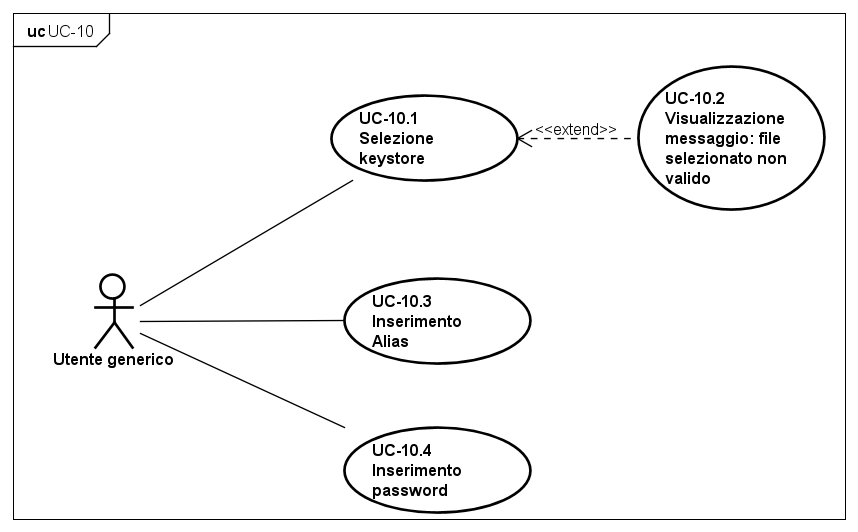
\includegraphics[width=10cm, height=8cm]{./immagini/usecase/uc_10.png}
    \caption{Sottocasi d'uso del caso d'uso UC-10.}
\end{figure}

\subsection*{UC-11 Visualizzazione credenziali keystore errati}\label{subsec:uc-11-visualizzazione-credenziali-keystore-errati}
\begin{itemize}
    \item \textbf{attori:} utente generico;
    \item \textbf{descrizione:} per firmare l'APK l'utente deve inserire delle credenziali, e quando quest'ultime sono errate viene mostrato un messaggio di errore;
    \item \textbf{pre-condizioni:} l'utente ha selezionato la funzionalità per ricompilare l'APK;
    \item \textbf{post-condizioni:} l'utente ha visualizzato il messaggio di errore;
    \item \textbf{flusso degli eventi principali:}
    \begin{itemize}
        \item l'utente ha visualizzato l'errore;
    \end{itemize}
\end{itemize}

\subsection*{UC-12 Visualizzazione messaggio file non valido}\label{subsec:uc-12-visualizzazione-messaggio-file-non-valido}
\begin{itemize}
    \item \textbf{attori:} utente generico;
    \item \textbf{descrizione:} quando l'utente seleziona un file che non ha l'estensione APK un messaggio deve essere mostrato all'utente;
    \item \textbf{pre-condizioni:} l'utente ha selezionato un file non APK;
    \item \textbf{post-condizioni:} l'utente ha visualizzato il messaggio d'errore;
    \item \textbf{flusso degli eventi principali:}
    \begin{itemize}
        \item l'utente visualizza il messaggio d'errore.
    \end{itemize}
\end{itemize}
\subsection*{UC-13 Decodifica dei file \textit{.dex} in file \textit{.java}}\label{subsec:uc-13-decodifica-dei-filetextitin-filetextit}
\begin{itemize}
    \item \textbf{attori:} utente generico;
    \item \textbf{descrizione:} dall'APK ricompilato si ottengono dei file \textit{.dex} che possono essere convertiti in \textit{.class} e quindi in \textit{.java};
    \item \textbf{pre-condizioni:} la decompilazione dell'APK \`{e} andata a buon fine;
    \item \textbf{post-condizioni:} la decodifica dei file \textit{.dex} in \textit{.java} \`{e} andata a buon fine;
    \item \textbf{flusso degli eventi principali:}
    \begin{itemize}
        \item l'utente seleziona la voce "Decodifica Dex".
    \end{itemize}
\end{itemize}

\subsection*{UC-14 Analisi del codice \textit{.java}}\label{subsec:uc-14-analisi-del-codicetextit}
\begin{itemize}
    \item \textbf{attori:} attore generico;
    \item \textbf{descrizione:} dopo aver ottenuto i file \textit{.java} eseguendo il caso d'uso UC-13, si potr\`{a} effettuare dell'analisi sul codice;
    \item \textbf{pre-condizioni:} la decodifica dei file \textit{.dex} in \textit{.java} \`{e} andata a buon fine;
    \item \textbf{post-condizioni:} viene generato un pdf con i risultati dell'analisi;
    \item \textbf{flusso degli eventi principali:}
    \begin{itemize}
        \item l'utente seleziona la voce "analyze";
        \item selezione delle opzioni di analisi;
        \item il file viene salvato nel percorso specificato dall'utente.
    \end{itemize}
    \item \textbf{Estensione:}
    \begin{itemize}
        \item UC-14.1 Selezione path per salvare i risultati;
        \item UC-14.2 Elencare i file analizzati;
        \item UC-14.3 Trovare le stringhe hard-coded;
        \item UC-14.4 Selezionare un file black list;
        \item UC-14.5 Analizzare i dati dello storage interno;
        \item UC-14.6 Selezionare un file di white list.
    \end{itemize}
\end{itemize}
\begin{figure}[H]
    \centering
    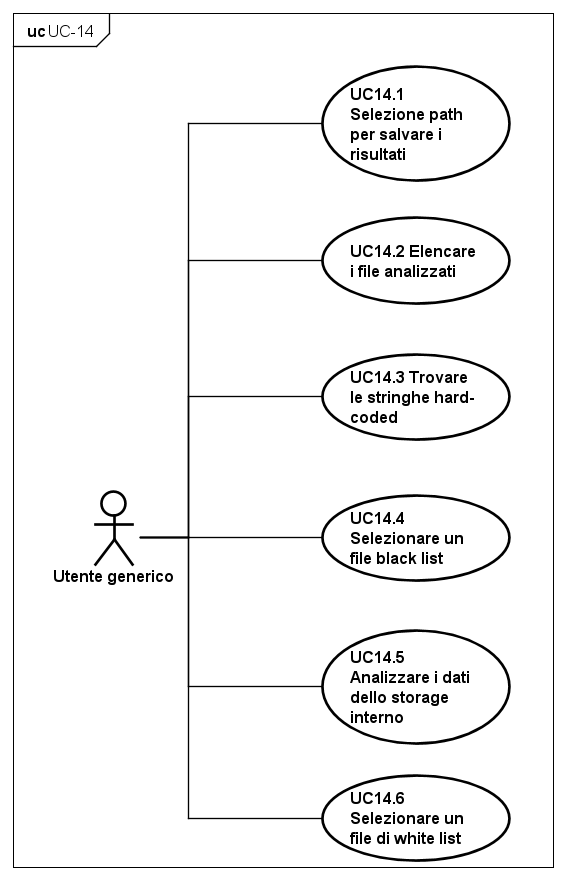
\includegraphics[width=10cm, height=12cm]{./immagini/usecase/subcases_14_1.png}
    \caption{Sottocasi d'uso del caso d'uso 14.}
\end{figure}

\subsection*{UC-14.1 Selezione path per salvare i risultati}
\begin{itemize}
    \item \textbf{attori:} attore generico;
    \item \textbf{descrizione:} l'utente deve specificare il path di destinazione del pdf che contiene i risultati dell'analisi;
    \item \textbf{pre-condizioni:} l'utente ha selezionato l'opzione di analisi del tool;
    \item \textbf{post-condizioni:} l'utente ha specificato il path di destinazione del pdf;
    \item \textbf{flusso degli eventi principali:}
    \begin{itemize}
        \item l'utente seleziona il path di destinazione.
    \end{itemize}
\end{itemize}
\subsection*{UC-14.2 Elencare i file analizzati}
\begin{itemize}
    \item \textbf{attori:} attore generico;
    \item \textbf{descrizione:} l'utente specifica che il pdf risultante deve contenere una lista dei file analizzati;
    \item \textbf{pre-condizioni:} l'utente ha selezionato l'opzione di analisi;
    \item \textbf{post-condizioni:} l'utente ha selezionato l'opzione di elencare i file analizzati;
    \item \textbf{flusso degli eventi principali:}
    \begin{itemize}
        \item l'utente seleziona l'opzione di elencare i file analizzati.
    \end{itemize}
\end{itemize}
\subsection*{UC-14.3 Trovare le stringhe hard-coded}
\begin{itemize}
    \item \textbf{attori:} attore generico;
    \item \textbf{descrizione:} l'utente specifica che il pdf risultante deve contenere tutte le stringhe hard-coded presenti nei codici sorgenti analizzati;
    \item \textbf{pre-condizioni:} l'utente ha selezionato l'opzione di analisi;
    \item \textbf{post-condizioni:}; l'utente ha selezionato l'opzione per trovare le stringhe hard-coded presenti nei codici sorgenti;
    \item \textbf{flusso degli eventi principali:}
    \begin{itemize}
        \item l'utente seleziona la voce Trovare le stringhe hard-coded.
    \end{itemize}
\end{itemize}
\subsection*{UC-14.4 Selezionare un file blacklist}
\begin{itemize}
    \item \textbf{attori:} attore generico;
    \item \textbf{descrizione:} l'utente seleziona un file di blacklist;
    \item \textbf{pre-condizioni:} l'utente ha selezionato l'opzione di analisi;
    \item \textbf{post-condizioni:} l'utente ha selezionato un file di blacklist;
    \item \textbf{flusso degli eventi principali:}
    \begin{itemize}
        \item l'utente inserisce il file path verso il file di blacklist.
    \end{itemize}
\end{itemize}
\subsection*{UC-14.5 Analizzare i dati dello storage interno}
\begin{itemize}
    \item \textbf{attori:} attore generico;
    \item \textbf{descrizione:} l'utente seleziona la voce analisi dei dati presenti nell'area dello storage dell'app;
    \item \textbf{pre-condizioni:} l'utente ha selezionato l'opzione di analisi;
    \item \textbf{post-condizioni:} l'utente ha selezionato la voce di analisi dei dati dati dell'area dello storage;
    \item \textbf{flusso degli eventi principali:}
    \begin{itemize}
        \item l'utente ha selezionato la voce analisi dei dati presenti nell'area dello storage dell'app.
    \end{itemize}
\end{itemize}
\subsection*{UC-14.6 Selezionare un file whitelist}
\begin{itemize}
    \item \textbf{attori:} attore generico;
    \item \textbf{descrizione:} l'utente seleziona un file di whitelist;
    \item \textbf{pre-condizioni:} l'utente ha selezionato l'opzione di analisi;
    \item \textbf{post-condizioni:} l'utente ha selezionato un file di whitelist;
    \item \textbf{flusso degli eventi principali:}
    \begin{itemize}
        \item l'utente inserisce il file path verso il file di whitelist.
    \end{itemize}
\end{itemize}


\subsection*{UC-15 avvio AVD}\label{subsec:uc-15-avvio-avd}
\begin{itemize}
    \item \textbf{attori:} attore generico;
    \item \textbf{descrizione:} serve per avviare un'avd per poter eseguire l'applicazione;
    \item \textbf{pre-condizioni:} il tool è stato avviato correttamente e nel sistema è presente almeno un AVD;
    \item \textbf{post-condizioni:} l'AVD è stato avviato correttamente;
    \item \textbf{flusso degli eventi principali:}
    \begin{itemize}
        \item l'attore visualizza l'elenco delle AVD presenti nel sistema;
        \item l'attore seleziona un'AVD che vuole avviare;
        \item l'attore seleziona se utilizzare un proxy da impostare nell'AVD;
        \item l'attore seleziona la voce avvia AVD.
    \end{itemize}
    \item \textbf{estensione:} UC-5 Visualizzazione messaggio nessun AVD rilevato.
\end{itemize}
\subsection*{UC-16 avvio AVD senza proxy}\label{subsec:uc-16-avvio-avd-senza-proxy}
\begin{itemize}
    \item \textbf{attori:} attore generico;
    \item \textbf{descrizione:} quando l'attore decide che non vuole avviare l'AVD modificando le impostazioni di proxy, viene eseguito questo caso d'uso;
    \item \textbf{pre-condizioni:} l'attore ha avviato correttamente il tool e nel sistema è presente almeno un'AVD;
    \item \textbf{post-condizioni:} l'AVD è stato avviato correttamente con le impostazioni di proxy di default;
    \item \textbf{flusso degli eventi principali:}
    \begin{itemize}
        \item l'attore visualizza l'elenco delle AVD presenti nel sistema;
        \item l'attore seleziona un'AVD che vuole avviare;
        \item l'attore seleziona di non utilizzare un proxy da impostare nell'AVD;
        \item l'attore seleziona la voce avvia AVD.
    \end{itemize}
\end{itemize}
\subsection*{UC-17 avvio AVD con proxy}\label{subsec:uc-16-avvio-avd-con-proxy}
\begin{itemize}
    \item \textbf{attori:} attore generico;
    \item \textbf{descrizione:} quando l'attore decide che non vuole avviare l'AVD modificando le impostazioni di proxy, viene eseguito questo caso d'uso;
    \item \textbf{pre-condizioni:} l'attore ha avviato correttamente il tool e nel sistema è presente almeno un'AVD;
    \item \textbf{post-condizioni:} l'AVD è stato avviato correttamente con le impostazioni di proxy inseriti;
    \item \textbf{flusso degli eventi principali:}
    \begin{itemize}
        \item l'attore visualizza l'elenco delle AVD presenti nel sistema;
        \item l'attore seleziona un'AVD che vuole avviare;
        \item l'attore seleziona di utilizzare un proxy da impostare nell'AVD;
        \item l'attore inserisce le informazioni del proxy, per esempio: \textit{localhost:8080};
        \item l'attore seleziona la voce avvia AVD.
    \end{itemize}
\end{itemize}
\subsubsection*{UC-17.1 Selezione voce Avvia con proxy}
\begin{itemize}
    \item \textbf{attori:} attore generico;
    \item \textbf{descrizione:} l'utente vuole avviare l'AVD con le opzioni di proxy;
    \item \textbf{pre-condizioni:} il tool è stato avviato correttamente ed è riuscito a rilevare gli AVD presenti nel sistema;
    \item \textbf{post-condizioni:} l'opzione di proxy è stata selezionata;
    \item \textbf{flusso degli eventi principali:}
    \begin{itemize}
        \item l'utente seleziona la voce per avviare l'AVD.
    \end{itemize}
\end{itemize}
\subsubsection*{UC-17.2 selezione voce avvio AVD}
\begin{itemize}
    \item \textbf{attori:} attore generico;
    \item \textbf{descrizione:} l'utente avvia l'AVD;
    \item \textbf{pre-condizioni:} l'utente ha selezionato le opzioni per avviare l'AVD;
    \item \textbf{post-condizioni:} il tool avvia l'AVD;
    \item \textbf{flusso degli eventi principali:}
    \begin{itemize}
        \item l'utente seleziona la voce avvio l'AVD.
    \end{itemize}
\end{itemize}
\subsubsection*{UC-17.3 inserimento indirizzo e porta proxy}
\begin{itemize}
    \item \textbf{attori:} attore generico;
    \item \textbf{descrizione:} serve all'attore per inserire i dati del proxy;
    \item \textbf{pre-condizioni:} l'utente ha selezionato l'opzione di avviare l'AVD con il proxy;
    \item \textbf{post-condizioni:} i dati sono stati inseriti correttamente;
    \item \textbf{flusso degli eventi principali:}
    \begin{itemize}
        \item l'utente inserisce l'indirizzo IP del server proxy;
        \item l'utente inserisce il numero della porta del server proxy.
    \end{itemize}
\end{itemize}
\subsubsection*{UC-17.4 conferma dei dati}
\begin{itemize}
    \item \textbf{attori:} attore generico;
    \item \textbf{descrizione:} serve all'utente per confermare i dati inseriti per avviare l'AVD;
    \item \textbf{pre-condizioni:} l'utente ha inserito le opzioni di proxy correttamente;
    \item \textbf{post-condizioni:} l'AVD è stato avviato correttamente con le opzioni di proxy;
    \item \textbf{flusso degli eventi principali:}
    \begin{itemize}
        \item l'utente conferma le informazioni inserite e avvia l'AVD.
    \end{itemize}
\end{itemize}

\begin{figure}[H]
    \centering
    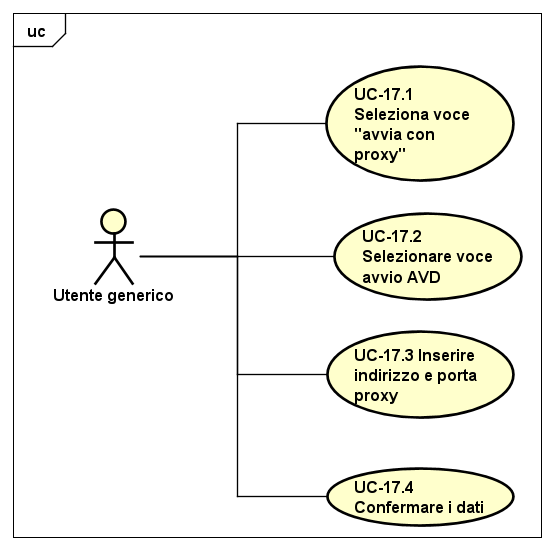
\includegraphics[width=10cm, height=8cm]{./immagini/usecase/uc_17.png}
    \caption{Sottocasi d'uso del caso d'uso 17.}
\end{figure}
\subsection*{UC-18 Inizio registrazione traffico di rete}\label{subsec:uc-18-inizio-registrazione-traffico-di-rete}
\begin{itemize}
    \item \textbf{attori:} attore generico;
    \item \textbf{descrizione:} quando l'utente vuole registrare le attività di rete effettuate dall'AVD eseguendo l'applicazione, può utilizzare questa funzionalità;
    \item \textbf{pre-condizioni:} l'attore ha avviato l'applicazione;
    \item \textbf{post-condizioni:} l'attore ha registrato le attività di rete e ottenuto un file pcap;
    \item \textbf{flusso degli eventi principali:}
    \begin{itemize}
        \item l'attore seleziona la voce "Start record!";
        \item l'attore successivamente seleziona la voce "Stop Record".
    \end{itemize}
\end{itemize}
\begin{figure}[H]
    \centering
    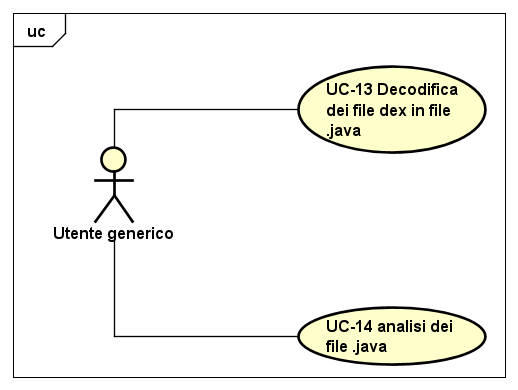
\includegraphics[width=10cm, height=8cm]{./immagini/usecase/UC-13_14.png}
    \caption{Casi d'uso da 13 a 18.}
\end{figure}

%\subsection*{UC-}
%\begin{itemize}
%    \item \textbf{attori:} attore generico;
%    \item \textbf{descrizione:}
%    \item \textbf{pre-condizioni:}
%    \item \textbf{post-condizioni:}
%    \item \textbf{flusso degli eventi principali:}
%    \begin{itemize}
%    \end{itemize}
%\end{itemize}